\documentclass[tikz,border=10pt]{standalone}
\usepackage{tikz}
\usetikzlibrary{shapes,arrows,positioning,calc,fit,backgrounds}
\usepackage{amsmath}

\begin{document}

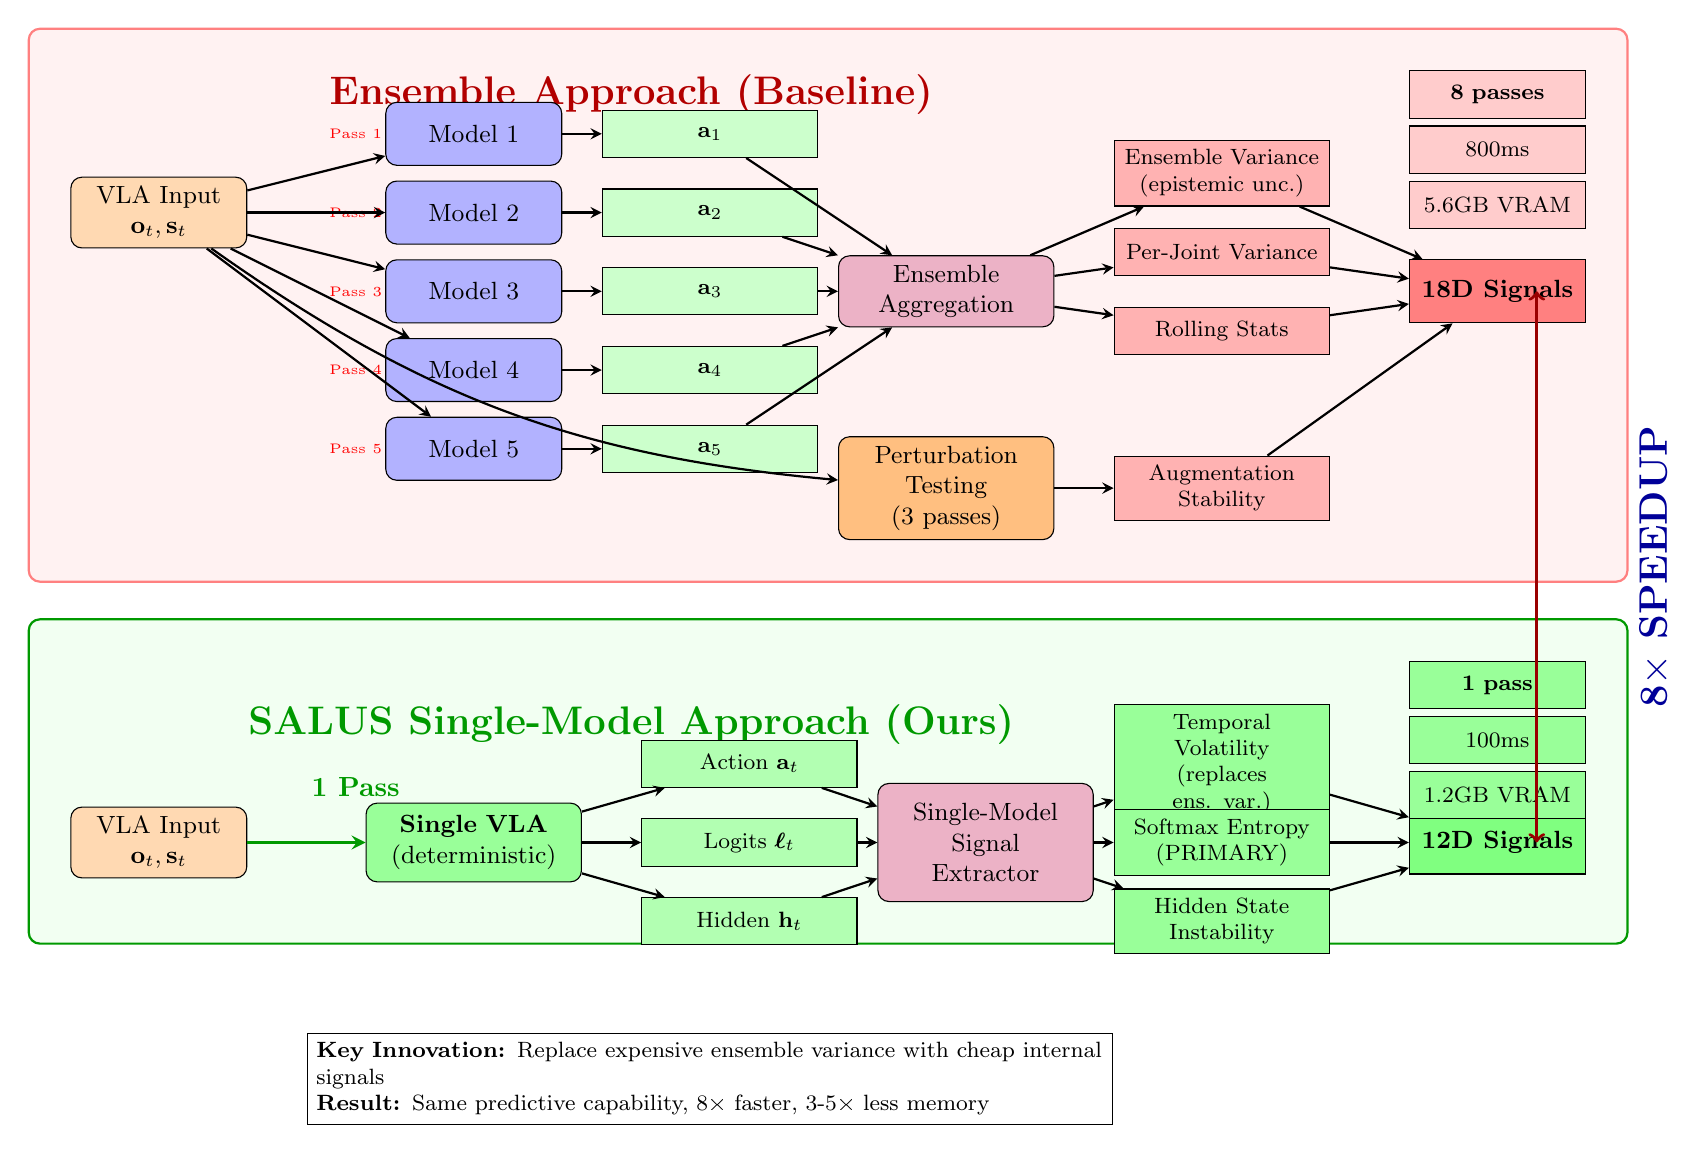
\begin{tikzpicture}[
    model/.style={rectangle, draw, fill=blue!30, text width=2cm, text centered, rounded corners, minimum height=0.8cm, font=\small},
    signal/.style={rectangle, draw, fill=green!20, text width=2.5cm, text centered, minimum height=0.6cm, font=\footnotesize},
    metric/.style={rectangle, draw, fill=yellow!30, text width=2cm, text centered, minimum height=0.6cm, font=\footnotesize},
    arrow/.style={thick,->,>=stealth}
]

% ============================================================
% ENSEMBLE APPROACH (OLD) - TOP HALF
% ============================================================

\node[font=\Large\bfseries, color=red!70!black] at (0, 10) {Ensemble Approach (Baseline)};

% Input
\node[model, fill=orange!30] (input_old) at (-6, 8.5) {VLA Input\\$\mathbf{o}_t, \mathbf{s}_t$};

% 5 Models
\node[model] (m1) at (-2, 9.5) {Model 1};
\node[model] (m2) at (-2, 8.5) {Model 2};
\node[model] (m3) at (-2, 7.5) {Model 3};
\node[model] (m4) at (-2, 6.5) {Model 4};
\node[model] (m5) at (-2, 5.5) {Model 5};

% Forward pass labels
\node[font=\tiny, color=red] at (-3.5, 9.5) {Pass 1};
\node[font=\tiny, color=red] at (-3.5, 8.5) {Pass 2};
\node[font=\tiny, color=red] at (-3.5, 7.5) {Pass 3};
\node[font=\tiny, color=red] at (-3.5, 6.5) {Pass 4};
\node[font=\tiny, color=red] at (-3.5, 5.5) {Pass 5};

% Arrows to models
\draw[arrow] (input_old) -- (m1);
\draw[arrow] (input_old) -- (m2);
\draw[arrow] (input_old) -- (m3);
\draw[arrow] (input_old) -- (m4);
\draw[arrow] (input_old) -- (m5);

% Actions
\node[signal] (a1) at (1, 9.5) {$\mathbf{a}_1$};
\node[signal] (a2) at (1, 8.5) {$\mathbf{a}_2$};
\node[signal] (a3) at (1, 7.5) {$\mathbf{a}_3$};
\node[signal] (a4) at (1, 6.5) {$\mathbf{a}_4$};
\node[signal] (a5) at (1, 5.5) {$\mathbf{a}_5$};

\draw[arrow] (m1) -- (a1);
\draw[arrow] (m2) -- (a2);
\draw[arrow] (m3) -- (a3);
\draw[arrow] (m4) -- (a4);
\draw[arrow] (m5) -- (a5);

% Aggregation
\node[model, fill=purple!30, text width=2.5cm] (agg) at (4, 7.5) {Ensemble\\Aggregation};

\draw[arrow] (a1) -- (agg);
\draw[arrow] (a2) -- (agg);
\draw[arrow] (a3) -- (agg);
\draw[arrow] (a4) -- (agg);
\draw[arrow] (a5) -- (agg);

% Signals from ensemble
\node[signal, fill=red!30] (sig_ens1) at (7.5, 9) {Ensemble Variance\\(epistemic unc.)};
\node[signal, fill=red!30] (sig_ens2) at (7.5, 8) {Per-Joint Variance};
\node[signal, fill=red!30] (sig_ens3) at (7.5, 7) {Rolling Stats};

\draw[arrow] (agg) -- (sig_ens1);
\draw[arrow] (agg) -- (sig_ens2);
\draw[arrow] (agg) -- (sig_ens3);

% Perturbation testing (3 extra passes)
\node[model, fill=orange!50, text width=2.5cm] (pert) at (4, 5) {Perturbation\\Testing\\(3 passes)};
\node[signal, fill=red!30] (sig_pert) at (7.5, 5) {Augmentation\\Stability};

\draw[arrow] (input_old) to[bend right=15] (pert);
\draw[arrow] (pert) -- (sig_pert);

% 18D output
\node[signal, fill=red!50, text width=2cm, minimum height=0.8cm, font=\small\bfseries] (output_old) at (11, 7.5) {18D Signals};

\draw[arrow] (sig_ens1) -- (output_old);
\draw[arrow] (sig_ens2) -- (output_old);
\draw[arrow] (sig_ens3) -- (output_old);
\draw[arrow] (sig_pert) -- (output_old);

% Metrics for old approach
\node[metric, fill=red!20] (metric1) at (11, 10) {\textbf{8 passes}};
\node[metric, fill=red!20] (metric2) at (11, 9.3) {800ms};
\node[metric, fill=red!20] (metric3) at (11, 8.6) {5.6GB VRAM};

% Box around ensemble approach
\begin{scope}[on background layer]
\node[draw=red!50, thick, rounded corners, fill=red!5, fit=(input_old) (m1) (m5) (agg) (pert) (output_old) (metric1) (metric3), inner sep=15pt] {};
\end{scope}

% ============================================================
% SINGLE-MODEL APPROACH (NEW) - BOTTOM HALF
% ============================================================

\node[font=\Large\bfseries, color=green!60!black] at (0, 2) {SALUS Single-Model Approach (Ours)};

% Input
\node[model, fill=orange!30] (input_new) at (-6, 0.5) {VLA Input\\$\mathbf{o}_t, \mathbf{s}_t$};

% Single model
\node[model, fill=green!40, text width=2.5cm, minimum height=1cm] (model_new) at (-2, 0.5) {\textbf{Single VLA}\\(deterministic)};

% Forward pass label
\node[font=\small, color=green!60!black, font=\bfseries] at (-3.5, 1.2) {1 Pass};

\draw[arrow, very thick, green!60!black] (input_new) -- (model_new);

% Extracted components
\node[signal, fill=green!30] (action_new) at (1.5, 1.5) {Action $\mathbf{a}_t$};
\node[signal, fill=green!30] (logits_new) at (1.5, 0.5) {Logits $\boldsymbol{\ell}_t$};
\node[signal, fill=green!30] (hidden_new) at (1.5, -0.5) {Hidden $\mathbf{h}_t$};

\draw[arrow] (model_new) -- (action_new);
\draw[arrow] (model_new) -- (logits_new);
\draw[arrow] (model_new) -- (hidden_new);

% Signal extractor
\node[model, fill=purple!30, text width=2.5cm, minimum height=1.5cm] (extractor) at (4.5, 0.5) {Single-Model\\Signal\\Extractor};

\draw[arrow] (action_new) -- (extractor);
\draw[arrow] (logits_new) -- (extractor);
\draw[arrow] (hidden_new) -- (extractor);

% New signals
\node[signal, fill=green!40] (sig_new1) at (7.5, 1.5) {Temporal Volatility\\(replaces ens. var.)};
\node[signal, fill=green!40] (sig_new2) at (7.5, 0.5) {Softmax Entropy\\(PRIMARY)};
\node[signal, fill=green!40] (sig_new3) at (7.5, -0.5) {Hidden State\\Instability};

\draw[arrow] (extractor) -- (sig_new1);
\draw[arrow] (extractor) -- (sig_new2);
\draw[arrow] (extractor) -- (sig_new3);

% 12D output
\node[signal, fill=green!50, text width=2cm, minimum height=0.8cm, font=\small\bfseries] (output_new) at (11, 0.5) {12D Signals};

\draw[arrow] (sig_new1) -- (output_new);
\draw[arrow] (sig_new2) -- (output_new);
\draw[arrow] (sig_new3) -- (output_new);

% Metrics for new approach
\node[metric, fill=green!40] (metric_new1) at (11, 2.5) {\textbf{1 pass}};
\node[metric, fill=green!40] (metric_new2) at (11, 1.8) {100ms};
\node[metric, fill=green!40] (metric_new3) at (11, 1.1) {1.2GB VRAM};

% Box around single-model approach
\begin{scope}[on background layer]
\node[draw=green!60!black, thick, rounded corners, fill=green!5, fit=(input_new) (model_new) (extractor) (output_new) (metric_new1) (metric_new3), inner sep=15pt] {};
\end{scope}

% ============================================================
% COMPARISON ARROWS
% ============================================================

\draw[<->, very thick, red!60!black] (11.5, 7.5) -- (11.5, 0.5);
\node[rotate=90, font=\Large\bfseries, color=blue!60!black] at (13, 4) {8$\times$ SPEEDUP};

% Labels
\node[draw, fill=white, text width=10cm, font=\footnotesize, align=left] at (1, -2.5) {
    \textbf{Key Innovation:} Replace expensive ensemble variance with cheap internal signals\\
    \textbf{Result:} Same predictive capability, 8× faster, 3-5× less memory
};

\end{tikzpicture}

\end{document}
